
\documentclass{exam}

\usepackage{units} 
\usepackage{graphicx}
\usepackage[fleqn]{amsmath}
\usepackage{cancel}
\usepackage{float}
\usepackage{mdwlist}
\usepackage{booktabs}
\usepackage{cancel}
\usepackage{polynom}
\usepackage{caption}
\usepackage{fullpage}
\usepackage{xfrac}
\usepackage{enumerate}

\newcommand{\degree}{\ensuremath{^\circ}} 
\everymath{\displaystyle}

% \begin{figure}[H]
%   \centering
%   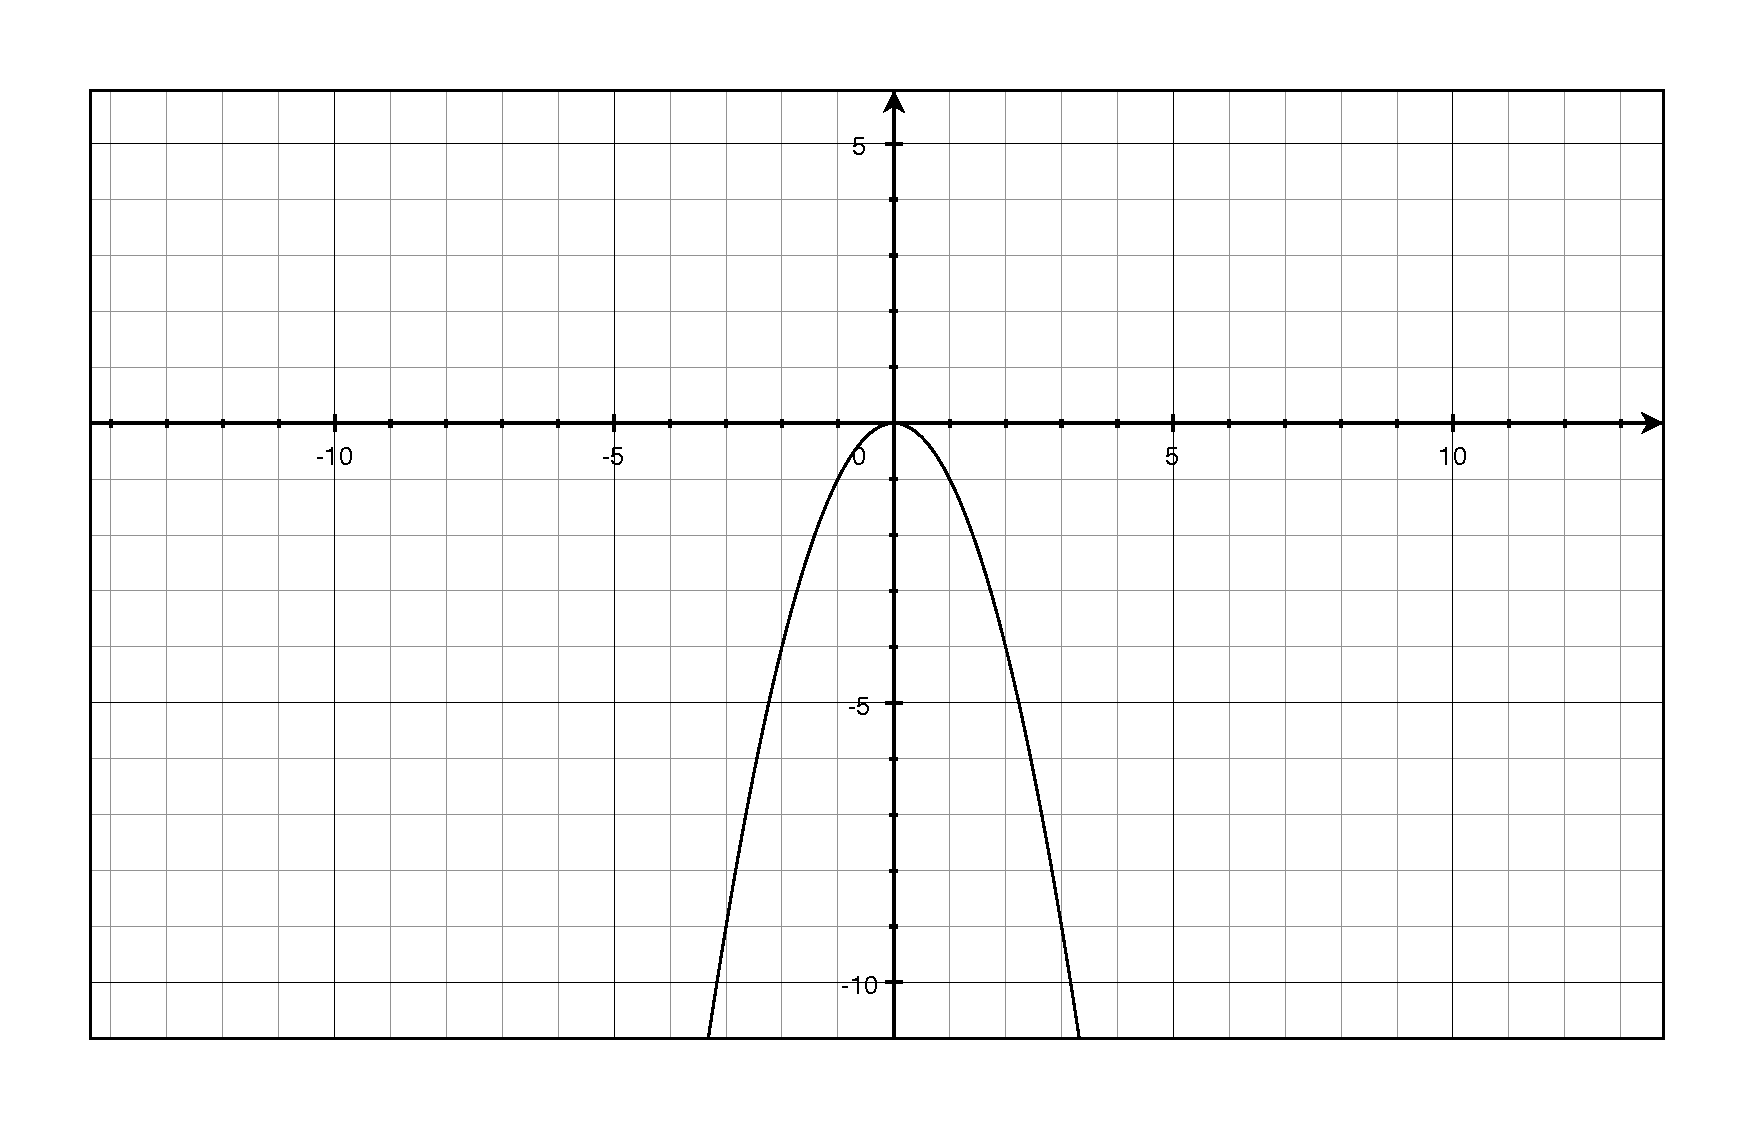
\includegraphics[scale=.3]{problem7.eps}
%   \caption*{Problem 7}
% \end{figure}

% \begin{tabular}{cc}
% \toprule
% period & amplitude \\
% \midrule
% value one & value two
% \bottomrule
% \end{tabular}

\printanswers

\ifprintanswers 
  \usepackage{2in1, lscape} 
\fi

\date{April 10, 2013}
\author{}
\title{Math 141 \\ Homework 8}

\begin{document}

  \maketitle

  \section{Homework}

  \begin{itemize*}
    \item Read Section 3.2
    \item Section 3.2: 1-12, 17-22, 31-36, 40-44, 51-52, 57-58, 63-64
  \end{itemize*}

  \section{Extra Credit}
  Section 3.2, problem 67

  \ifprintanswers
    \begin{solution}
      It's usually easier to do the division than it is to evaluate large powers.  In this case, however, since the $x$
      value is $\pm 1$, it's easier to evaluate the polynomial than it is to do the division.  Evaluating the polynomial
      lets you use the {Remainder Theorem} in reverse to answer the questions.

      \begin{enumerate}[a]
        \item[a] 
          $P(-1) = 6 - 17 - 12 + 26 = 3$

          The remainder when dividing by $x + 1$ is 3.

        \item
          $P(1) = 1 - 3 + 1 + 2 = 1$

          Since $P(1) \neq 0$, $1$ is not a root and $x - 1$ is not a factor.

      \end{enumerate}

    \end{solution}

  \fi

  \section{Review}

  \begin{enumerate}

    \uplevel{For problems 1-2, find $f \circ g$, $g \circ f$, $f \circ f$, $g \circ g$}

    \item $f(x) = \sqrt{x - 1}$; $g(x) = x^2 - 4$
      \begin{solution}
        \begin{align*}
          (f \circ g)(x) &= \sqrt{x^2 - 5} \\
          (g \circ f)(x) &= x - 5 \\
          (f \circ f)(x) &= \sqrt{\sqrt{x - 1} - 1} \\
          (g \circ g)(x) &= x^4 - 8x^2 + 12 \\
        \end{align*}
      \end{solution}

    \item $f(x) = \frac{2x}{x - 1}$; $g(x) = 3x + 1$
      \begin{solution}
        \begin{align*}
          (f \circ g)(x) &= \frac{6x + 2}{3x} \\
          (g \circ f)(x) &= \frac{7x - 1}{x - 1} \\
          (f \circ f)(x) &= \frac{4x}{x + 1} \\
          (g \circ g)(x) &= 9x + 4 \\
        \end{align*}
      \end{solution}

    \ifprintanswers
      \pagebreak
    \fi

    \item 
      The lengths of the sides of a cube with side length $x$ are increasing at $\unitfrac[2]{m}{s}$.

      \begin{enumerate}[a]
        \item What is the function that models the side length as a function of time?
          \begin{solution}
            \[ \boxed{s(t) = x + 2t} \]
          \end{solution}

        \item Find a function that models the surface area as a function of time.
          \begin{solution}
              The surface area of a cube is $S(x) = 6x^2$, so the function is 
              \[
                (S \circ x)(t) = 6 (x + 2t)^2 = \boxed{\unitfrac[24t^2 + 24tx + 6x^2]{m^2}{s}}
              \]
          \end{solution}

        \item Find a function that models the volume as a function of time.
          \begin{solution}
              The volume of a cube is $V(x) = x^3$, so the function is 
              \[
                (V \circ x)(t) = (x + 2t)^3 = \boxed{\unitfrac[8t^3 + 12t^2x + 6tx^2 + x^3]{m^3}{s}}
              \]
          \end{solution}

      \end{enumerate}

  \end{enumerate}

  \ifprintanswers

  \pagebreak

    \section{Section 3.2}

    \begin{description}

      \item[1]
        \[
          \polyhornerscheme[x = -3]{3x^2 + 5x - 4}
        \]

        \[
          3x^2 + 5x - 4 = \boxed{(3x - 4)(x + 3) + 8}
        \]

      \item[2] 
        \[
          \polyhornerscheme[x = 1]{x^3 + 4x^2 - 6x + 1}
        \]

        \[
          x^3 + 4x^2 - 6x + 1 = \boxed{\left( x^2 + 5x - 1 \right)(x - 1)}
        \]

      \item[3] 
        \[
          \polylongdiv{2x^3 - 3x^2 - 2x}{2x - 3}
        \]

        \[
          2x^3 - 3x^2 - 2x = \boxed{\left( x^2 - 1 \right) (2 x - 3) - 3}
        \]

      \item[4] 
        \[
          \polylongdiv{4x^3 + 7x + 9}{2x + 1}
        \]

        \[
          4x^3 + 7x + 9 = \boxed{\left( 2x^2 - x + 4 \right) (2 x + 1) + 5}
        \]

      \item[5] 
        \[
          \polylongdiv{x^4 - x^3 + 4x + 2}{x^2 + 3}
        \]

        \[
          x^4 - x^3 + 4x + 2 = \boxed{\left( x^2 - x - 3 \right) (x^2 + 3) + 7x + 11}
        \]

      \pagebreak

      \item[6] 
        \[
          \polylongdiv{2x^5 + 4x^4 - 4x^3 - x - 3}{x^2 - 2}
        \]

        \[
          2x^5 + 4x^4 - 4x^3 - x - 3 = \boxed{\left( 2x^3 + 4x^2 + 8 \right)(x^2 - 2) + 13 - x}
        \]

      \item[7] 
        \[
          \polyhornerscheme[x = -3]{x^2 + 4x - 8}
        \]

        \[
          \frac{x^2 + 4x - 8}{x + 3} = \boxed{x + 1 - \frac{11}{x + 3}}
        \]

      \item[8] 
        \[
          \polyhornerscheme[x = 4]{x^3 + 6x + 5}
        \]

        \[
          \frac{x^3 + 6x + 5}{x - 4} = \boxed{x^2 + 4x + 22 + \frac{93}{x - 4}}
        \]

      \pagebreak

      \item[9] 
        \[
          \polylongdiv{4x^2 - 3x - 7}{2x - 1}
        \]

        \[
          \frac{4x^2 - 3x - 7}{2x - 1} = \boxed{2x - \frac{1}{2} - \frac{15}{2(2x - 1)}}
        \]

      \item[10] 
        \[
          \polylongdiv{6x^3 + x^2 - 12x + 5}{3x - 4}
        \]

        \[
          \frac{6x^3 + x^2 - 12x + 5}{3x - 4} = \boxed{2x^2 + 3x + \frac{5}{3x - 4}}
        \]

      \item[11] 
        \[
          \polylongdiv{2x^4 - x^3 + 9x^2}{x^2 + 4}
        \]

        \[
          \frac{2x^4 - x^3 + 9x^2}{x^2 + 4} = \boxed{2x^2 - x + 1 + \frac{4x - 4}{x^2 + 4}}
        \]

      \item[12] 
        \[
          \polylongdiv{x^5 + x^4 - 2x^3 + x + 1}{x^2 + x - 1}
        \]

        \[
          \frac{x^5 + x^4 - 2x^3 + x + 1}{x^2 + x - 1} = \boxed{x^3 - x + 1 + \frac{2- x}{x^2 + x - 1}}
        \]

      \item[17] 
        \[
          \polylongdiv{x^3 + 6x + 3}{x^2 - 2x + 2}
        \]

      \item[18] 
        \[
          \polylongdiv{3x^4 - 5x^3 - 20x - 5}{x^2 + x + 3}
        \]

      \item[19] 
        \[
          \polylongdiv{6x^3 + 2x^2 + 22x}{2x^2 + 5}
        \]

      \item[20] 
        \[
          \polylongdiv{9x^2 - x + 5}{3x^2 - 7x}
        \]

      \item[21] 
        \[
          \polylongdiv{x^6 + x^4 + x^2 + 1}{x^2 + 1}
        \]

      \item[22] 
        \[
          \polylongdiv{2x^5 - 7x^4 - 13}{4x^2 - 6x + 8}
        \]

      \item[31] 
        \[
          \polyhornerscheme[x = 1]{x^5 + 3x^3 - 6}
        \]

        \fbox{$x^4 + x^3 + 4x^2 + 4x + 4$ remainder $-2$}

      \item[32] 
        \[
          \polyhornerscheme[x = 3]{x^3 - 9x^2 + 27x - 27}
        \]

        \fbox{$x^2 - 6x + 9$ remainder $0$}

      \item[33] 
        \[
          \polyhornerscheme[x = \frac{1}{2}]{2x^3 + 3x^2 - 2x + 1}
        \]

        \fbox{$2x^2 + 4x$ remainder $1$}

      \item[34] 
        \[
          \polyhornerscheme[x = -\frac{2}{3}]{6x^4 + 10x^3 + 5x^2 + x + 1}
        \]

        \fbox{$6x^3 + 6x^2 + x + \frac{1}{3}$ remainder $\frac{7}{9}$}

      \pagebreak

      \item[35] 
        \[
          \polyhornerscheme[x = 3]{x^3 - 27}
        \]

        \fbox{$x^2 + 3x + 9$ remainder $0$}

      \item[36] 
        \[
          \polyhornerscheme[x = -2]{x^4 - 16}
        \]

        \fbox{$x^3 - 2x^2 + 4x - 8$ remainder $0$}

      \item[40] 
        \[
          \polyhornerscheme[x = -1]{x^3 - x^2 + x + 5}
        \]

        \fbox{$P(-1) = 2$}

      \item[41] 
        \[
          \polyhornerscheme[x = -2]{x^3 + 2x^2 - 7}
        \]

        \fbox{$P(-2) = -7$}

      \item[42]
        \[
          \polyhornerscheme[x = 11]{2x^3 - 21x^2 + 9x - 200}
        \]

        \fbox{$P(11) = 20$}

      \item[43]
        \[
          \polyhornerscheme[x = -7]{5x^4 + 30x^3 - 40x^2 + 36x + 14}
        \]

        \fbox{$P(-7) = -483$}

      \item[44]
        \[
          \polyhornerscheme[x = -2]{6x^5 + 10x^3 + x + 1}
        \]

        \fbox{$P(-2) = -273$}

      \item[51]
        \[
          \polyhornerscheme[x = 1]{x^3 - 3x^2 + 3x - 1}
        \]

      \item[52]
        \[
          \polyhornerscheme[x = 2]{x^3 + 2x^2 - 3x - 10}
        \]

      \item[57]
        \begin{align*}
          P(x) &= (x + 1)(x - 1)(x - 3) \\
          &= (x^2 - 1)(x - 3) \\
          &= \boxed{x^3 - 3x^2 - x + 3} \\
        \end{align*}

      \item[58]
        \begin{align*}
          P(x) &= (x + 2)x(x - 2)(x - 4) \\
               &= x(x^2 - 4)(x - 4) \\
               &= \boxed{x^4 - 4x^3 - 4x^2 + 16x} \\
        \end{align*}

      \item[63]
        First find a polynomial with the correct zeros:
        \begin{align*}
          P(x) &= a(x + 1)(x - 1)(x - 2) \\
               &= a(x^3 - 2x^2 - x + 2) \\
        \end{align*}

        $a$ is the constant that determines how much the graph is scaled in the y direction.  Since $P(0) = 2$:
        \begin{align*}
          2 &= 2a \\
          a &= 1 \\
        \end{align*}

        The final polynomial is: \fbox{$P(x) = x^3 - 2x^2 - x + 2$}

      \item[64]
        First find a polynomial with the correct zeros.  The $(x - 1)$ term is squared since the graph just touches the
        $x$ axis and changes direction at that point.

        \begin{align*}
          P(x) &= a(x + 1)(x - 2)^2 \\
               &= a(x^3 - 3x^2 + 4) \\
        \end{align*}

        $a$ is the constant that determines how much the graph is scaled in the y direction.  Since $P(0) = 4$:
        \begin{align*}
          4 &= 4a \\
          a &= 1 \\
        \end{align*}

        The final polynomial is: \fbox{$P(x) = x^3 - 3x^2 + 4$}

    \end{description}
  \else
    \vspace{3 cm}
    \begin{em}
      The point of public relations slogans like ``Support Our Troops'' is that they don't mean anything \ldots that's
      the whole point of good propaganda. You want to create a slogan that nobody is going to be against and I suppose
      everybody will be for, because nobody knows what it means, because it doesn't mean anything. But its crucial value
      is that it diverts your attention from a question that does mean something, do you support our policy? And that's
      the one you're not allowed to talk about.
    \end{em}

    \hspace{1 cm} --Noam Chomsky
  \fi

\end{document}

